\section*{Đề thi thử THPTQG Sở GD\&ĐT SƠN LA 25-26, Lần 2}

\caulc
\Opensolutionfile{ans}[ans/ans-26-2--SoGD-L1-LC]

\begin{ex} %Câu 1. %[1D5H1-3]
	Doanh thu bán hàng trong $20$ ngày được lựa chọn ngẫu nhiên của một cửa hàng được ghi lại ở bảng sau (đơn vị: triệu đồng):
	\begin{center}
		\begin{tabular}{|c|c|c|c|c|c|}
			\hline
			Doanh thu & $[5;7)$ & $[7;9)$ & $[9;11)$ & $[11;13)$ & $[13;15)$ \\
			\hline
			Số ngày & $2$ & $7$ & $7$ & $3$ & $1$ \\
			\hline
		\end{tabular}
	\end{center}
	Số trung bình của mẫu số liệu trên thuộc khoảng nào trong các khoảng dưới đây?
	\choice
	{$[7;9)$}
	{\True $[9;11)$}
	{$[11;13)$}
	{$[13;15)$}
	\loigiai
	{
		Ta có bảng giá trị đại diện:\\
		\begin{center}
			\begin{tabular}{|c|c|c|c|c|c|}
				\hline
				Doanh thu & $[5;7)$ & $[7;9)$ & $[9;11)$ & $[11;13)$ & $[13;15)$ \\
				\hline
				Giá trị đại diện & $6$ & $8$ & $10$ & $12$ & $14$ \\
				\hline
				Số ngày & $2$ & $7$ & $7$ & $3$ & $1$ \\
				\hline
			\end{tabular}
		\end{center}
		$\displaystyle \bar{x} = \frac{6 \cdot 2 + 8 \cdot 7 + 10 \cdot 7 + 12 \cdot 3 + 14 \cdot 1}{2+7+7+3+1} = \frac{12+56+70+36+14}{20} = \frac{188}{20} = 9{,}4$.\\
		Giá trị $9{,}4$ nằm trong khoảng $[9;11)$.
	}
\end{ex}

\begin{ex} %Câu 2. %[1H8H7-3]
	Cho hình chóp đều $S.ABCD$ có cạnh đáy bằng $a\sqrt{2}$, cạnh bên bằng $2a$. Thể tích khối chóp $S.ABCD$ là
	\choice
	{$\displaystyle \frac{4a^3}{3}$}
	{$\displaystyle \frac{a^3}{3}$}
	{\True $\displaystyle \frac{2a^3\sqrt{3}}{3}$}
	{$\displaystyle \frac{2a^3}{3}$}
	\loigiai
	{
		\begin{center}
			\begin{tikzpicture}[scale=1.0, line join=round, line cap=round]
				\coordinate (D) at (-2,-1.5);
				\coordinate (C) at (2,-1.5);
				\coordinate (B) at (4,0);
				\coordinate (A) at (0,0);
				\coordinate (S) at (1,2.5);
				\coordinate (O) at ($(B)!0.5!(D)$);
				\draw (B)--(C)--(D);
				\draw[dashed] (A)--(C);
				\draw[dashed] (B)--(D);
				\draw[dashed] (S)--(A);
				\draw (S)--(B);
				\draw (S)--(C);
				\draw (S)--(D);
				\draw[dashed] (B)--(A)--(D);
				\draw[dashed] (S)--(O);
				\node[left] at (A) {$A$};
				\node[below] at (B) {$B$};
				\node[right] at (C) {$C$};
				\node[above] at (D) {$D$};
				\node[below] at (O) {$O$};
				\node[above] at (S) {$S$};
			\end{tikzpicture}
		\end{center}
		Vì $S.ABCD$ là chóp đều nên đáy $ABCD$ là hình vuông cạnh $a\sqrt{2}$.\\
		Suy ra $\displaystyle S_{ABCD} = (a\sqrt{2})^2 = 2a^2$.\\
		Gọi $O$ là tâm hình vuông $ABCD$.\\
		Đường chéo $\displaystyle AC = \sqrt{(a\sqrt{2})^2 + (a\sqrt{2})^2} = \sqrt{4a^2} = 2a \Rightarrow OA = \frac{AC}{2} = a$.\\
		Xét tam giác vuông $SOA$ vuông tại $O$, ta có:\\
		$\displaystyle h = SO = \sqrt{SA^2 - OA^2} = \sqrt{(2a)^2 - a^2} = \sqrt{3a^2} = a\sqrt{3}$.\\
		Như vậy, thể tích $\displaystyle V = \frac{1}{3} \cdot 2a^2 \cdot a\sqrt{3} = \frac{2a^3\sqrt{3}}{3}$.
	}
\end{ex}

\begin{ex} %Câu 3. %[1H8N2-2]
	Cho hình chóp $S.ABCD$ có đáy là hình bình hành tâm $O$, $SA = SC$, $SB = SD$. Trong các khẳng định sau khẳng định nào đúng?
	\choice
	{\True $SO \perp (ABCD)$}
	{$SC \perp (ABCD)$}
	{$SB \perp (ABCD)$}
	{$SA \perp (ABCD)$}
	\loigiai
	{
		\begin{center}
			\begin{tikzpicture}[scale=1.0, line join=round, line cap=round]
				\coordinate (B) at (0,0);
				\coordinate (C) at (4,0);
				\coordinate (A) at (1.5,1.5);
				\coordinate (D) at ($(A)+(C)-(B)$);
				\coordinate (O) at ($(A)!0.5!(C)$);
				\coordinate (S) at ($(O)+(0,3)$);
				\draw (B) -- (C) -- (D) -- (S) -- (B);
				\draw (S) -- (C);
				\draw[dashed] (A) -- (B);
				\draw[dashed] (A) -- (D);
				\draw[dashed] (S) -- (A);
				\draw[dashed] (A) -- (C);
				\draw[dashed] (B) -- (D);
				\draw[dashed] (S) -- (O);
				\node[left] at (A) {$A$};
				\node[below left] at (B) {$B$};
				\node[below right] at (C) {$C$};
				\node[right] at (D) {$D$};
				\node[below] at (O) {$O$};
				\node[above] at (S) {$S$};
			\end{tikzpicture}
		\end{center}
		Đáy $ABCD$ là hình bình hành tâm $O \Rightarrow OA = OC$ và $OB = OD$.\\
		Vì $SA = SC \Rightarrow \Delta SAC$ cân tại $S$. Do đó, $SO$ là đường cao của $\Delta SAC \colon SO \perp AC$.\\
		Vì $SB = SD \Rightarrow \Delta SBD$ cân tại $S$. Do đó, $SO$ là đường cao của $\Delta SBD \colon SO \perp BD$.\\
		Ta có: $\begin{cases} SO \perp AC \\ SO \perp BD \\ AC \cap BD = O \end{cases}$, suy ra $SO \perp (ABCD)$.
	}
\end{ex}

\begin{ex} %Câu 4. %[2H5N1-2]
	Trong không gian $Oxyz$, vectơ nào sau đây là vectơ pháp tuyến của mặt phẳng $(P) \colon 2x - y + z + 3 = 0$?
	\choice
	{\True $\vec{n_1} = (2;-1;1)$}
	{$\vec{n_3} = (2;-1;3)$}
	{$\vec{n_2} = (2;1;1)$}
	{$\vec{n_4} = (-1;1;3)$}
	\loigiai
	{
		Một vectơ pháp tuyến của mặt phẳng $(P)$ là $\vec{n} = (2;-1;1)$.
	}
\end{ex}

\begin{ex} %Câu 5. %[2D4N2-1]
	Cho $\displaystyle \int_0^1 f(x)\,dx = 1$ và $\displaystyle \int_0^2 f(x)\,dx = -4$. Tích phân $\displaystyle \int_1^2 f(x)\,dx$ bằng
	\choice
	{$3$}
	{$5$}
	{$-3$}
	{\True $-5$}
	\loigiai
	{
		Ta có: $\displaystyle \int_1^2 f(x)\,dx = \int_0^2 f(x)\,dx - \int_0^1 f(x)\,dx = -4 - 1 = -5$.
	}
\end{ex}

\begin{ex} %Câu 6. %[2D1N2-2]
	Cho hàm số $y = f(x)$ có đồ thị như hình vẽ.
	\begin{center}
		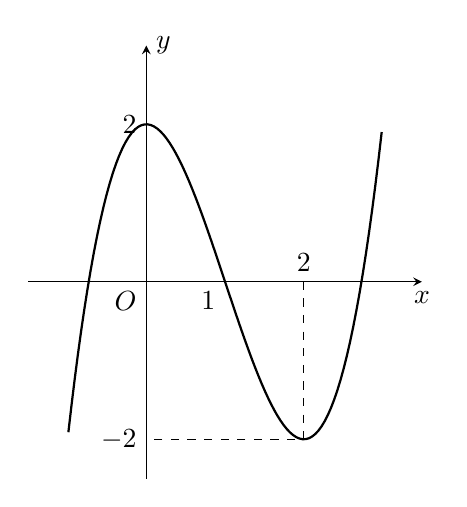
\begin{tikzpicture}[scale=1.0, >=stealth]
			\draw[->] (-1.5,0) -- (3.5,0) node[below] {$x$};
			\draw[->] (0,-2.5) -- (0,3) node[right] {$y$};
			\node[below left] at (0,0) {$O$};
			\draw[dashed] (2,0) -- (2,-2) -- (0,-2);
			\node[above] at (2,0) {$2$};
			\node[left] at (0,-2) {$-2$};
			\node[left] at (0,2) {$2$};
			\node[below left] at (1,0) {$1$};
			\draw[thick, domain=-0.99:2.99, samples=100] plot (\x, {(\x)^3 - 3*(\x)^2 + 2});
		\end{tikzpicture}
	\end{center}
	Điểm cực tiểu của hàm số đó là
	\choice
	{$x = -2$}
	{\True $x = 2$}
	{$x = 0$}
	{$y = -2$}
	\loigiai
	{
		Điểm cực tiểu của hàm số trên là $x = 2$.
	}
\end{ex}

\begin{ex} %Câu 7. %[2D4N1-3]
	Họ tất cả các nguyên hàm của hàm số $f(x) = \sin x$ là
	\choice
	{$-\sin x + C$}
	{$\sin x + C$}
	{\True $-\cos x + C$}
	{$\cos x + C$}
	\loigiai
	{
		Họ tất cả các nguyên hàm của hàm số $f(x) = \sin x$ là $-\cos x + C$.
	}
\end{ex}

\begin{ex} %Câu 8. %[2H5N3-2]
	Trong không gian $Oxyz$, cho mặt cầu $(S) \colon (x-2)^2 + (y+1)^2 + (z-3)^2 = 4$. Tâm của $(S)$ có tọa độ là
	\choice
	{$(-2;1;-3)$}
	{$(-4;2;-6)$}
	{$(4;-2;6)$}
	{\True $(2;-1;3)$}
	\loigiai
	{
		Tâm của mặt cầu $(S) \colon (x-2)^2 + (y+1)^2 + (z-3)^2 = 4$ có tọa độ là $(2;-1;3)$.
	}
\end{ex}

\begin{ex} %Câu 9. %[2D1H3-1]
	Giá trị lớn nhất của hàm số $f(x) = x^4 - 2x^2 + 5$ trên đoạn $[-2;2]$ là
	\choice
	{\True $\displaystyle \max_{[-2;2]} f(x) = 13$}
	{$\displaystyle \max_{[-2;2]} f(x) = 14$}
	{$\displaystyle \max_{[-2;2]} f(x) = -4$}
	{$\displaystyle \max_{[-2;2]} f(x) = 23$}
	\loigiai
	{
		$f'(x) = 4x^3 - 4x = 0 \Leftrightarrow \left[\begin{array}{l} x = 0 \\ x = 1 \\ x = -1 \end{array}\right.$.\\
		Cả $3$ nghiệm $x=0, x=1, x=-1$ đều thuộc đoạn $[-2;2]$.\\
		$f(-2) = 13$, $f(-1) = 4$, $f(0) = 5$, $f(1) = 4$, $f(2) = 13$.\\
		So sánh các kết quả trên, ta thấy giá trị lớn nhất là $13$.
	}
\end{ex}

\begin{ex} %Câu 10. %[2D1N4-1]
	Tiệm cận ngang của đồ thị hàm số $\displaystyle y = \frac{4x+1}{x-1}$ là
	\choice
	{$y = 2$}
	{$x = 1$}
	{\True $y = 4$}
	{$x = 4$}
	\loigiai
	{
		Đường tiệm cận ngang là $\displaystyle y = \frac{4}{1} = 4$.
	}
\end{ex}

\begin{ex} %Câu 11. %[1D9N1-3]
	Cho hai biến cố độc lập $A$, $B$. Biết $\displaystyle P(A) = \frac{1}{5}$, $\displaystyle P(B) = \frac{2}{3}$. $P(AB)$ bằng
	\choice
	{$\displaystyle \frac{13}{15}$}
	{\True $\displaystyle \frac{2}{15}$}
	{$\displaystyle \frac{3}{5}$}
	{$\displaystyle \frac{11}{15}$}
	\loigiai
	{
		Do hai biến cố $A$ và $B$ độc lập nên $\displaystyle P(AB) = P(A)P(B) = \frac{1}{5} \cdot \frac{2}{3} = \frac{2}{15}$.
	}
\end{ex}

\begin{ex} %Câu 12. %[1D2N2-4]
	Cho cấp số cộng $(u_n)$ có số hạng đầu $u_1 = 2$ và công sai $d = 5$. Giá trị của $u_4$ bằng
	\choice
	{$12$}
	{$22$}
	{$250$}
	{\True $17$}
	\loigiai
	{
		$u_4 = u_1 + 3d \Leftrightarrow u_4 = 2 + 3 \cdot 5 = 2 + 15 = 17$.
	}
\end{ex}
\Closesolutionfile{ans}


\cauds
\Opensolutionfile{ans}[ans/ans-26-2--SoGD-L1-DS]
\begin{ex} %Câu 1. %[2D1C5-4]
	Cho hàm số $\displaystyle y = f(x) = \frac{ax^2 + bx + c}{x + d}$ có đồ thị là đường cong như hình vẽ.
	\begin{center}
		\begin{tikzpicture}[>=stealth, scale=0.8]
			% Giới hạn khung hình để đồ thị không bị tràn khi x tiến gần 2
			\clip (-4,-5) rectangle (6,5);
			
			% Vẽ trục hoành Ox và trục tung Oy
			\draw[->] (-3.5,0) -- (5.5,0) node[above] {$x$};
			\draw[->] (0,-4.65) -- (0,4.5) node[right] {$y$};
			\node[below left] at (0,0) {$O$};
			
			% Đường tiệm cận đứng x = 2
			\draw[solid] (2,-4.65) -- (2,4.5);
			\node[below left] at (2,0) {$2$};
			
			% Đường tiệm cận xiên y = -x
			\draw[solid, domain=-3.7:4.7] plot (\x, {-\x});
			
			% Vẽ đồ thị hàm số nhánh bên trái (x < 2)
			\draw[thick, smooth, samples=100, domain=-3.5:1.15] 
			plot (\x, {(-\x*\x + 2*\x + 3) / (\x - 2)});
			
			% Vẽ đồ thị hàm số nhánh bên phải (x > 2)
			\draw[thick, smooth, samples=100, domain=2.43:5.5] 
			plot (\x, {(-\x*\x + 2*\x + 3) / (\x - 2)});
			
			% Đánh dấu các giao điểm với trục tọa độ
			\fill (3,0) circle (1.5pt) node[below right] {$3$};
			\fill (-1,0) circle (1.5pt) node[below left] {$-1$};
			\fill (0,-1.5) circle (1.5pt) node[left] {$-\frac{3}{2}$};
			
		\end{tikzpicture}
	\end{center}
	\choiceTF
	{Đạo hàm của hàm số $y = f(x)$ luôn dương $\forall x \in \mathbb{R} \setminus \{2\}$}
	{\True Tổng của hai hệ số $c$ và $d$ bằng $1$}
	{\True Đồ thị hàm số $y = f(x)$ có tiệm cận xiên là đường thẳng $y = -x$}
	{\True Để đường thẳng $y = m$ cắt đồ thị hàm số $y = f(x)$ tại hai điểm phân biệt $A$ và $B$ sao cho $OA \perp OB$ thì $m$ là nghiệm của phương trình $m^2 - 2m - 3 = 0$}
	\loigiai
	{
		\begin{itemchoice}
			\itemch Dựa vào đồ thị hàm số nghịch biến nên đạo hàm của hàm số $y = f(x)$ luôn âm $\forall x \in \mathbb{R} \setminus \{2\}$. Chọn SAI.
			\itemch Đồ thị hàm số đi qua $\left(0; -\frac{3}{2}\right) \Rightarrow \frac{c}{d} = -\frac{3}{2} \Rightarrow c = -\frac{3}{2}d$.\\
			Ta có tiệm cận đứng $x = 2 \Rightarrow d = -2 \Rightarrow c = 3$.\\
			Khi đó $c + d = 1$. Chọn ĐÚNG.
			\itemch Đồ thị hàm số đi qua $(-1; 0)$ và $(3; 0)$ suy ra\\
			$\begin{cases} 0 = \frac{a - b + 3}{-1 - 2} \\ 0 = \frac{9a + 3b + 3}{3 - 2} \end{cases} \Leftrightarrow \begin{cases} a - b = -3 \\ 3a + b = -1 \end{cases} \Leftrightarrow \begin{cases} a = -1 \\ b = 2 \end{cases}$.\\
			$\displaystyle \Rightarrow y = f(x) = \frac{-x^2 + 2x + 3}{x - 2} = -x + \frac{3}{x - 2}$.\\
			Tiệm cận xiên là $y = -x$. Chọn ĐÚNG.
			\itemch Xét phương trình $\displaystyle f(x) = m \Leftrightarrow \frac{-x^2 + 2x + 3}{x - 2} = m$, ĐK $x \neq 2$.\\
			$\displaystyle \frac{-x^2 + 2x + 3}{x - 2} = m \Rightarrow x^2 + (m - 2)x - 3 - 2m = 0$ (*)\\
			Phương trình (*) có $\Delta = (m + 2)^2 + 12 > 0 \, \forall m$, nên nó luôn có hai nghiệm phân biệt.\\
			Để đồ thị hàm số $y = f(x)$ cắt đường thẳng $y = m$ tại hai điểm phân biệt thì $m \neq \frac{7}{2}$.\\
			$A(x_1; m), B(x_2; m) \Rightarrow OA \perp OB \Leftrightarrow x_1 \cdot x_2 + m^2 = 0 \Leftrightarrow -3 - 2m + m^2 = 0 \Leftrightarrow m^2 - 2m - 3 = 0$. Chọn ĐÚNG.
		\end{itemchoice}
	}
\end{ex}

\begin{ex} %Câu 2. %[2D6V2-4]
	Trước thềm cuộc bầu cử đại biểu Hội đồng nhân dân ở tỉnh $X$, một cuộc trưng cầu dân ý online đã được tổ chức. Kết quả cho thấy có $40\%$ cử tri tham gia trả lời sẽ bầu cử cho ứng cử viên $A$. Sau cuộc bầu cử, tất cả cử tri từng tham gia cuộc trưng cầu dân ý online đều phản hồi lại kết quả mình đã bầu chọn. Các phản hồi cho thấy trong số các cử tri từng trả lời sẽ bầu cho ứng cử viên $A$ có $90\%$ đã thực sự bầu, trong số các cử tri từng trả lời sẽ không bầu cho ứng cử viên $A$ có $20\%$ đã bầu cho ứng cử viên $A$. Nếu chỉ xét những người tham gia cuộc trưng cầu dân ý online thì
	\choiceTF
	{\True Xác suất cử tri bầu ứng viên $A$ biết rằng trước bầu cử họ trả lời sẽ bầu ứng cử viên $A$ là $0{,}9$}
	{Xác suất cử tri không bầu ứng viên $A$ biết rằng trước bầu cử họ trả lời sẽ không bầu ứng cử viên $A$ là $0{,}2$}
	{\True Tỉ lệ cử tri bầu cho ứng cử viên $A$ là $48\%$}
	{Biết rằng một cử tri đã bầu cho ứng cử viên $A$, xác suất để họ đã nói sẽ không bầu ứng cử viên $A$ trước bầu cử là $0{,}2$}
	\loigiai
	{
		\begin{itemchoice}
			\itemch Gọi $M$ là biến cố "Cử tri trả lời sẽ bầu cho ứng cử viên $A$ trước cuộc bầu cử".\\
			Gọi $A$ là biến cố "Cử tri thực sự bầu cho ứng cử viên $A$".\\
			Xác suất cử tri bầu ứng viên $A$ biết rằng trước bầu cử họ trả lời sẽ bầu ứng cử viên $A$ là $P(A|M)$.\\
			Trong số những người trả lời sẽ bầu, có $90\%$ đã thực sự bầu $\Rightarrow P(A|M) = 90\% = 0{,}9$. Chọn ĐÚNG.
			\itemch Gọi $\overline{M}$ là biến cố đối của $M$: "Cử tri trả lời sẽ không bầu cho ứng cử viên $A$ trước cuộc bầu cử".\\
			Gọi $\overline{A}$ là biến cố đối của $A$: "Cử tri thực sự không bầu cho ứng cử viên $A$".\\
			Ta có $20\%$ cử tri từng trả lời sẽ không bầu cho ứng cử viên $A$ thực sự bầu cho ứng cử viên $A \Rightarrow P(A|\overline{M}) = 20\% = 0{,}2$.\\
			Xác suất cử tri không bầu ứng viên $A$ biết rằng trước bầu cử họ trả lời sẽ không bầu ứng cử viên $A$ là $P(\overline{A}|\overline{M})$.\\
			Ta có: $P(\overline{A}|\overline{M}) = 1 - P(A|\overline{M}) = 1 - 0{,}2 = 0{,}8$. Chọn SAI.
			\itemch Xác suất cử tri trả lời sẽ bầu cho ứng cử viên $A$ trước cuộc bầu cử là: $P(M) = 40\% = 0{,}4$.\\
			$\Rightarrow P(\overline{M}) = 1 - P(M) = 1 - 0{,}4 = 0{,}6$.\\
			Tỉ lệ cử tri thực sự bầu cho ứng cử viên $A$ là:\\
			$P(A) = P(M) \cdot P(A|M) + P(\overline{M}) \cdot P(A|\overline{M}) = 0{,}4 \cdot 0{,}9 + 0{,}6 \cdot 0{,}2 = 0{,}48 = 48\%$. Chọn ĐÚNG.
			\itemch Xác suất để cử tri trả lời sẽ không bầu cho ứng cử viên $A$ trước cuộc bầu cử nhưng thực sự bầu cho ứng cử viên $A$ là: $P(\overline{M}|A)$.\\
			Ta có: $\displaystyle P(\overline{M}|A) = \frac{P(\overline{M}) \cdot P(A|\overline{M})}{P(A)} = \frac{0{,}6 \cdot 0{,}2}{0{,}48} = 0{,}25$. Chọn SAI.
		\end{itemchoice}
	}
\end{ex}

\begin{ex} %Câu 3. %[2H5V3-2]
	Trong không gian $Oxyz$ cho mặt cầu $(S) \colon x^2 + (y-2)^2 + (z+1)^2 = 29$, hai điểm $A(0; 0; 4)$, $B(6; -2; 6)$ và đường thẳng $\displaystyle d \colon \frac{x-4}{1} = \frac{y+8}{-1} = \frac{z-4}{2}$. Gọi $M$ điểm thuộc mặt cầu $(S)$ sao cho $\widehat{AMB} = 90^\circ$.
	\choiceTF
	{\True Điểm $A$ nằm trên mặt cầu $(S)$ và điểm $B$ nằm ngoài mặt cầu $(S)$}
	{Đường thẳng $d$ là tiếp tuyến của mặt cầu $(S)$}
	{\True Điểm $M$ nằm trên mặt phẳng $(P) \colon x - y + 2z - 8 = 0$}
	{Gọi $(a; b; c)$ là tọa độ của điểm $M$ khi khoảng cách từ điểm $M$ đến đường thẳng $d$ ngắn nhất. Giá trị của biểu thức $T = a^2 + b^2 + c^2$ bằng $10$}
	\loigiai
	{
		\begin{itemchoice}
			\itemch Mặt cầu $(S)$ có tâm $I(0; 2; -1)$ và bán kính $R = \sqrt{29}$.\\
			Ta có $IA = \sqrt{(-2)^2 + 5^2} = \sqrt{29} = R$, suy ra điểm $A$ nằm trên mặt cầu $(S)$.\\
			$IB = \sqrt{(-6)^2 + 4^2 + (-5)^2} = \sqrt{77} > R$, suy ra điểm $B$ nằm ngoài mặt cầu $(S)$. Chọn ĐÚNG.
			\itemch $d$ đi qua điểm $E(4; -8; 4)$ và có $\vec{u} = (1; -1; 2)$.\\
			Ta có $\overrightarrow{IE} = (4; -10; 5)$, $[\vec{u}, \overrightarrow{IE}] = (15; 3; -6)$.\\
			Khi đó $\displaystyle d(I, d) = \frac{|[\vec{u}, \overrightarrow{IE}]|}{|\vec{u}|} = \frac{\sqrt{15^2 + 3^2 + (-6)^2}}{\sqrt{1^2 + (-1)^2 + 2^2}} = 3\sqrt{5} \neq R$.\\
			Vậy đường thẳng $d$ không là tiếp tuyến của mặt cầu $(S)$. Chọn SAI.
			\itemch Ta có $\widehat{AMB} = 90^\circ$ nên điểm $M$ thuộc mặt cầu $(S_1)$ có đường kính $AB$.\\
			Gọi $J$ là trung điểm $AB$, suy ra $J(3; -1; 5)$ là tâm $(S_1)$, bán kính $\displaystyle R_1 = \frac{AB}{2} = \sqrt{11}$.\\
			Khi đó $(S_1) \colon (x - 3)^2 + (y + 1)^2 + (z - 5)^2 = 11$.\\
			Tọa độ điểm $M$ thỏa mãn hệ phương trình\\
			$\begin{cases} x^2 + (y - 2)^2 + (z + 1)^2 = 29 \\ (x - 3)^2 + (y + 1)^2 + (z - 5)^2 = 11 \end{cases} \Leftrightarrow x - y + 2z - 8 = 0$.\\
			Vậy điểm $M$ nằm trên mặt phẳng $(P) \colon x - y + 2z - 8 = 0$. Chọn ĐÚNG.
			\itemch 
			Gọi $H$ là tâm đường tròn nên $H$ là hình chiếu của $I$ lên $(P)$.\\
			Gọi $N = d \cap (P)$.\\
			Khi đó khoảng cách từ điểm $M$ đến đường thẳng $d$ ngắn nhất thì $M$ thuộc đoạn $NH$.\\
			$d(I, (P)) = 2\sqrt{6}$.\\
			$IH \colon \begin{cases} x = t \\ y = 2 - t \\ z = -1 + 2t \end{cases} \Rightarrow H(t; 2 - t; -1 + 2t)$.\\
			$\Rightarrow IH^2 = 6t^2 = 24 \Rightarrow \left[\begin{array}{l} t = 2 \Rightarrow H(2; 0; 3) \\ t = -2 \Rightarrow H(-2; 4; -5) \end{array}\right.$.\\
			Do $H \in (P)$ nên $H(2; 0; 3)$.\\
			$N = d \cap (P) \Rightarrow N(4 + t; -8 - t; 4 + 2t)$\\
			$N \in (P) \Rightarrow 4 + t - (-8 - t) + 2(4 + 2t) - 8 = 0 \Leftrightarrow t = -2 \Rightarrow N(2; -6; 0)$.\\
			Khi đó, $NH = 3\sqrt{5}$ và $MH = \sqrt{IM^2 - IH^2} = \sqrt{5}$.\\
			Ta có $\overrightarrow{MH} = (2 - a; -b; 3 - c)$ và $\overrightarrow{NH} = (0; 6; 3)$.\\
			$\Rightarrow \overrightarrow{NH} = 3\overrightarrow{MH} \Rightarrow \begin{cases} 3(2 - a) = 0 \\ -3b = 6 \\ 3(3 - c) = 3 \end{cases} \Leftrightarrow \begin{cases} a = 2 \\ b = -2 \\ c = 2 \end{cases}$.\\
			Vậy $M(2; -2; 2)$, suy ra $T = a^2 + b^2 + c^2 = 12$. Chọn SAI.
		\end{itemchoice}
	}
\end{ex}

\begin{ex} %Câu 4. %[2D4V2-6]
	Một chất điểm chuyển động trên đường thẳng với vận tốc $v(t)$, $0 \le t \le 5$ ($t$ có đơn vị là giây và $v(t)$ có đơn vị mét/giây). Hàm số $v(t)$ có đồ thị gồm hai đoạn thẳng $OB$, $BC$ và đường cong $CD$ là một phần parabol $v(t) = at^2 + bt + c$ ($a, b, c \in \mathbb{R}$) có đỉnh $C$ (như hình vẽ).
	\begin{center}
		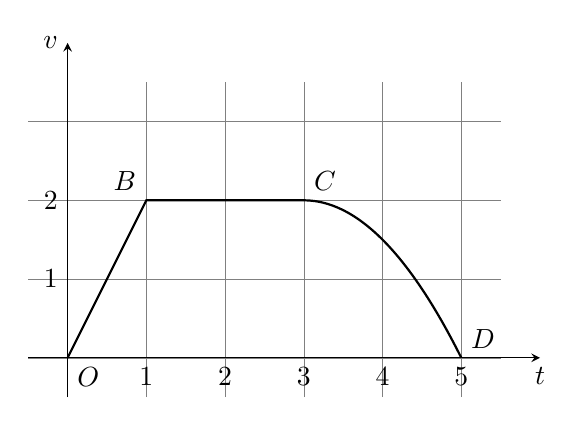
\begin{tikzpicture}[scale=1.0, >=stealth]
			\draw[help lines, step=1] (-0.5,-0.5) grid (5.5,3.5);
			\draw[->] (-0.5,0) -- (6,0) node[below] {$t$};
			\draw[->] (0,-0.5) -- (0,4) node[left] {$v$};
			\node[below right] at (0,0) {$O$};
			\node[below] at (1,0) {$1$};
			\node[below] at (2,0) {$2$};
			\node[below] at (3,0) {$3$};
			\node[below] at (4,0) {$4$};
			\node[below] at (5,0) {$5$};
			\node[left] at (0,1) {$1$};
			\node[left] at (0,2) {$2$};
			\draw[thick] (0,0) -- (1,2) node[above left] {$B$} -- (3,2) node[above right] {$C$};
			\draw[thick, domain=3:5, samples=100] plot (\x, {-0.5*(\x-3)^2 + 2});
			\node[above right] at (5,0) {$D$};
		\end{tikzpicture}
	\end{center}
	\choiceTF
	{\True Trong một giây đầu tiên, vận tốc của chất điểm là $v(t) = 2t$, $0 \le t \le 1$}
	{\True Quãng đường chất điểm đi được trong hai giây đầu tiên là $3m$}
	{Giá trị của $a$ là $\displaystyle a = -\frac{5}{2}$}
	{Quãng đường chất điểm đi được trong khoảng thời gian bốn giây đầu tiên là $7{,}7m$ (làm tròn đến hàng phần mười)}
	\loigiai
	{
		\begin{itemchoice}
			\itemch Trong một giây đầu tiên, vận tốc của chất điểm là $v(t) = 2t$, $0 \le t \le 1$.\\
			Trong một giây đầu tiên, vận tốc của chất điểm có đồ thị là đường thẳng $v(t) = at + b$ đi qua hai điểm có toạ độ $(0; 0)$ và $(1; 2)$ nên $\begin{cases} a \cdot 0 + b = 0 \\ a \cdot 1 + b = 2 \end{cases} \Leftrightarrow \begin{cases} a = 2 \\ b = 0 \end{cases}$.\\
			Vậy, $v(t) = 2t$. Chọn ĐÚNG.
			\itemch Quãng đường chất điểm đi được trong hai giây đầu tiên là diện tích của hình thang $BMNO$:\\
			\begin{center}
				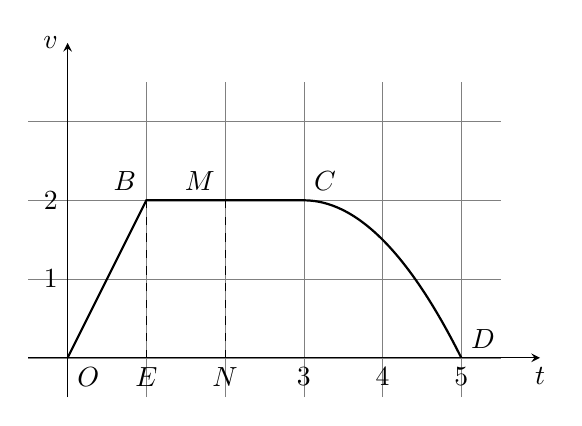
\begin{tikzpicture}[scale=1.0, >=stealth]
					\draw[help lines, step=1] (-0.5,-0.5) grid (5.5,3.5);
					\draw[->] (-0.5,0) -- (6,0) node[below] {$t$};
					\draw[->] (0,-0.5) -- (0,4) node[left] {$v$};
					\node[below right] at (0,0) {$O$};
					\node[below] at (1,0) {$E$};
					\node[below] at (2,0) {$N$};
					\node[below] at (3,0) {$3$};
					\node[below] at (4,0) {$4$};
					\node[below] at (5,0) {$5$};
					\node[left] at (0,1) {$1$};
					\node[left] at (0,2) {$2$};
					\draw[thick] (0,0) -- (1,2) node[above left] {$B$} -- (2,2) node[above left] {$M$} -- (3,2) node[above right] {$C$};
					\draw[thick, domain=3:5, samples=100] plot (\x, {-0.5*(\x-3)^2 + 2});
					\node[above right] at (5,0) {$D$};
					\draw[dashed] (1,0) -- (1,2);
					\draw[dashed] (2,0) -- (2,2);
				\end{tikzpicture}
			\end{center}
			$\displaystyle S_{BCFO} = S_{BEO} + S_{BMNE} = \frac{1}{2} \cdot 2 \cdot 1 + 1 \cdot 2 = 3$. Chọn ĐÚNG.
			\itemch $CD$ là một phần parabol $v(t) = at^2 + bt + c$.\\
			Parabol đi qua điểm $D(5; 0)$ và có đỉnh là điểm $C(3; 2)$ nên\\
			$\begin{cases} a \cdot 5^2 + b \cdot 5 + c = 0 \\ a \cdot 3^2 + b \cdot 3 + c = 2 \\ -\frac{b}{2a} = 3 \end{cases} \Leftrightarrow \begin{cases} 25a + 5b + c = 0 \\ 9a + 3b + c = 2 \\ b = -6a \end{cases} \Leftrightarrow \begin{cases} 25a - 30a + c = 0 \\ 9a - 18a + c = 2 \\ b = -6a \end{cases} \Leftrightarrow \begin{cases} -5a + c = 0 \\ -9a + c = 2 \\ b = -6a \end{cases} \Leftrightarrow \begin{cases} a = -\frac{1}{2} \\ b = 3 \\ c = -\frac{5}{2} \end{cases}$. Chọn SAI.
			\itemch Quãng đường chất điểm đi được trong khoảng thời gian bốn giây đầu tiên là:\\
			$\displaystyle v(t) = -\frac{1}{2}t^2 + 3t - \frac{5}{2}, t \ge 3$.\\
			Quãng đường chất điểm đi được trong khoảng thời gian bốn giây đầu tiên là\\
			$\displaystyle \frac{1}{2} \cdot 1 \cdot 2 + 2 \cdot 2 + \int_3^4 \left(-\frac{1}{2}t^2 + 3t - \frac{5}{2}\right)\,dt = 5 + \left(-\frac{1}{6}t^3 + \frac{3t^2}{2} - \frac{5}{2}t\right) \bigg|_3^4$\\
			$\displaystyle = 5 + \left(-\frac{1}{6} \cdot 4^3 + \frac{3 \cdot 4^2}{2} - \frac{5}{2} \cdot 4\right) - \left(-\frac{1}{6} \cdot 3^3 + \frac{3 \cdot 3^2}{2} - \frac{5}{2} \cdot 3\right) = 5 + \frac{10}{3} - \frac{3}{2} \approx 6{,}8$. Chọn SAI.
		\end{itemchoice}
	}
\end{ex}
\Closesolutionfile{ans}

\caukq
\Opensolutionfile{ans}[ans/ans-26-2--SoGD-L1-KQ]
\begin{ex} %Câu 1. %[2D1V3-6]
	Trong kế hoạch khai thác tuyến ca nô cao tốc phục vụ du lịch sinh thái trên vùng lòng hồ Thủy điện Sơn La (từ bến Mường La đi Quỳnh Nhai) có chiều dài $100\text{ km}$. Ban quản lý cần xác định vận tốc khai thác $v\text{ (km/h)}$ cho ca nô ($30 \le v \le 70$) để đạt lợi nhuận kinh tế cao nhất. Các thông số được xác định như sau: Công suất tiêu thụ điện của động cơ ca nô là $P(v) = 10v^3\text{ (W)}$. Giá điện kinh doanh tại bến sạc là $2000\text{ đồng/kWh}$. Chi phí vận hành cố định: Bao gồm nhân lực lái tàu, khấu hao và bến bãi, được tính là $2500000\text{ đồng}$ cho mỗi giờ ca nô chạy. Số lượng khách mua vé cho mỗi chuyến phụ thuộc vào vận tốc khai thác theo hàm số: $\displaystyle N(v) = \frac{v}{5} + 20$ (hành khách). Giá vé bình quân cho tuyến này là $500000\text{ đồng/khách}$. Hãy xác định vận tốc khai thác $v$ để lợi nhuận ròng của mỗi chuyến ca nô trên tuyến này là lớn nhất. (Biết công thức tính điện lượng tiêu thụ là $A = P(v) \cdot t$).
	\shortans[oly]{$50$}
	\loigiai
	{
		Thời gian ca nô di chuyển là: $\displaystyle t = \frac{100}{v}\text{ (giờ)}$.\\
		Điện năng tiêu thụ là: $\displaystyle A = P(v) \cdot t = \frac{v^3}{100} \cdot \frac{100}{v} = v^2\text{ (kWh)}$.\\
		Như vậy tiền điện sạc là: $2000v^2$.\\
		Chi phí vận hành là: $\displaystyle 2.500.000 \cdot \frac{100}{v} = \frac{250.000.000}{v}\text{ (đồng)}$.\\
		Vậy tổng chi phí cho một chuyến là: $\displaystyle C(v) = 2000v^2 + \frac{100}{v} \cdot 2500000\text{ (đồng)}$.\\
		Lợi nhuận thu được sau $1$ chuyến đi là:\\
		$\displaystyle L(v) = -2000v^2 + 100.000v + 10.000.000 - \frac{250.000.000}{v}\text{ (đồng)}$.\\
		Ta có: $\displaystyle L'(v) = -4000v + 100.000 + \frac{250.000.000}{v^2}$.\\
		$\displaystyle L'(v) = 0 \Leftrightarrow -4v^3 + 100v^2 + 250.000 = 0 \Leftrightarrow v = 50$.\\
		Ta có $\displaystyle L(v) = -2000v^2 + 100.000v + 10.000.000 - \frac{250.000.000}{v}$\\
		Ta có: $L(50) = 5000000$; $L(30) \approx 2866666{,}7$; $L(70) \approx 3628871{,}4$\\
		Vậy vận tốc $50\text{ (km/h)}$ thì lợi nhuận ròng của mỗi chuyến ca nô trên tuyến này là lớn nhất.
	}
\end{ex}

\begin{ex} %Câu 2. %[2D4V3-2]
	Một xưởng mộc tại Mai Sơn sản xuất những chiếc bàn cờ Ô quan bằng gỗ nguyên khối. Mặt trên của bàn cờ là một mặt phẳng được thiết kế và có kích thước như hình vẽ gồm ba phần: phần chính giữa là một hình chữ nhật có chiều dài $100\text{ cm}$ và chiều rộng $40\text{ cm}$; hai "ô quan" ở hai đầu trái và phải là hai hình phẳng bằng nhau được ghép nối liền mạch với hai cạnh chiều rộng của hình chữ nhật. Biết rằng đường bao ngoài của mỗi "ô quan" là một cung tròn. Xưởng mộc tiến hành phủ một lớp keo bảo vệ bóng lên toàn bộ bề mặt trên của chiếc bàn cờ này. Biết chi phí vật tư và nhân công để phủ keo là $100000\text{ đồng/m}^2$. Tính tổng chi phí $x$ (nghìn đồng) để hoàn thiện việc phủ keo cho mặt bàn cờ (Kết quả làm tròn đến hàng đơn vị).
	\begin{center}
		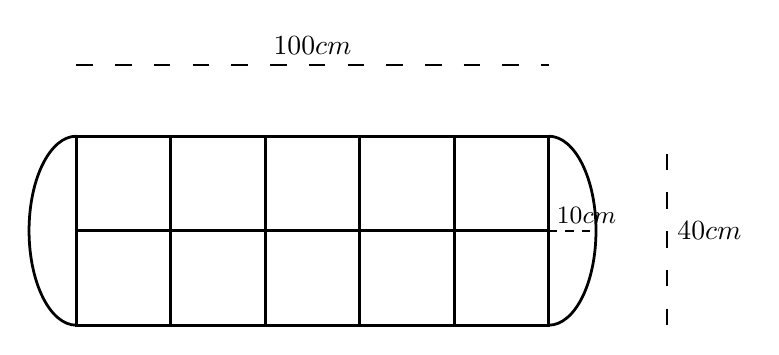
\begin{tikzpicture}[line width=1pt, scale=0.6]
			% Phần lưới hình chữ nhật ở giữa (các ô dân)
			\draw (0,0) rectangle (10,4);
			\draw (0,2) -- (10,2);
			\foreach \x in {2, 4, 6, 8} {
				\draw (\x,0) -- (\x,4);
			}
			
			% Hai cung elip ở hai đầu (hai ô quan)
			% Cung bên trái
			\draw (0,4) arc (90:270:1 and 2);
			% Cung bên phải
			\draw (10,4) arc (90:-90:1 and 2);
			
			% Đường đứt nét và nhãn "100 cm"
			\draw[dash pattern=on 6pt off 8pt, thick] (0,5.5) -- (10,5.5);
			\node[above] at (5,5.5) {$100 \text{ cm}$};
			
			% Đường đứt nét và nhãn "40 cm"
			\draw[dash pattern=on 6pt off 8pt, thick] (12.5,0) -- (12.5,4);
			\node[right] at (12.5,2) {$40 \text{ cm}$};
			
			% Đường đứt nét và nhãn "10 cm" bên trong ô quan phải
			\draw[dashed, thick] (10,2) -- (11,2);
			\node[above, inner sep=2pt] at (10.8,2) {\small $10 \text{ cm}$};
			
		\end{tikzpicture}
	\end{center}
	\shortans[oly]{$46$}
	\loigiai
	{
		\begin{center}
			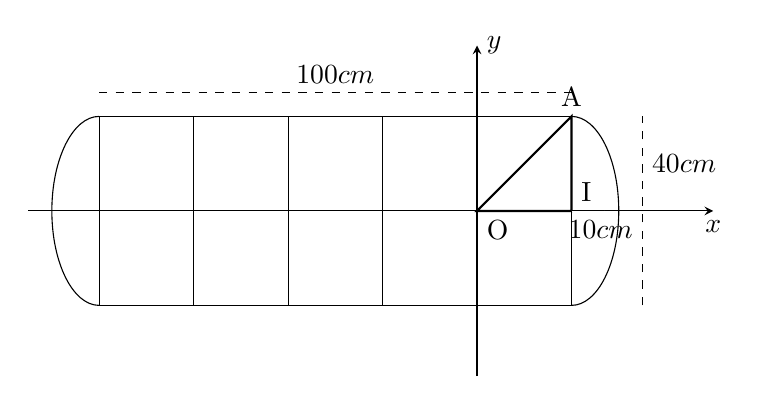
\begin{tikzpicture}[>=stealth, scale=0.06]
				% Định nghĩa các tham số giới hạn
				\def\Lx{-80} % Cạnh trái của lưới hình chữ nhật
				\def\Rx{20}  % Cạnh phải của lưới hình chữ nhật
				\def\Ty{20}  % Cạnh trên
				\def\By{-20} % Cạnh dưới
				
				% 1. Vẽ hệ trục tọa độ Oxy (vẽ dài ra ngoài hình)
				\draw[->] (\Lx-15, 0) -- (\Rx+30, 0) node[below] {$x$};
				\draw[->] (0, \By-15) -- (0, \Ty+15) node[right] {$y$};
				
				% 2. Vẽ lưới hình chữ nhật (5 ô ngang x 2 ô dọc)
				\draw (\Lx, \By) rectangle (\Rx, \Ty);
				% Các đường dọc bên trong
				\foreach \x in {-60, -40, -20} {
					\draw (\x, \By) -- (\x, \Ty);
				}
				% Đường dọc trùng với trục Oy (nét liền của lưới)
				\draw (0, \By) -- (0, \Ty);
				% Đường dọc tại x = 20 (chứa đoạn IA)
				\draw (\Rx, \By) -- (\Rx, \Ty);
				
				% 3. Vẽ hai nửa elip ở hai đầu
				% Nửa trái (tâm tại -80, bán trục x=10, trục y=20)
				\draw (\Lx, \Ty) arc (90:270:10 and 20);
				% Nửa phải (tâm tại 20, bán trục x=10, trục y=20)
				\draw (\Rx, \Ty) arc (90:-90:10 and 20);
				
				% 4. Vẽ tam giác vuông OIA bằng nét đậm
				\draw[thick] (0,0) -- (20,20) -- (20,0) -- cycle;
				
				% 5. Đánh dấu tên các điểm
				\node[below right] at (0,0) {O};
				\node[above] at (20,20) {A};
				\node[above right] at (20,0) {I};
				
				% 6. Vẽ các đường gióng đứt nét và ghi chú kích thước
				% Kích thước 100cm
				\draw[dashed] (\Lx, \Ty+5) -- (\Rx, \Ty+5);
				\node[above] at (-30, \Ty+5) {$100\text{cm}$};
				
				% Kích thước 40cm
				\draw[dashed] (\Rx+15, \By) -- (\Rx+15, \Ty);
				\node[right] at (\Rx+15, 10) {$40\text{cm}$};
				
				% Kích thước 10cm (Bán kính của elip bên phải)
				% Cố ý vẽ đứt nét đoạn từ I(20,0) đến mép elip (30,0) để giống ảnh
				\draw[dashed, thick, white] (20,0) -- (30,0); % Dùng nét trắng đè lên trục x
				\draw[dashed] (20,0) -- (30,0);
				\node[below, xshift=2pt] at (25, 0) {$10\text{cm}$};
				
			\end{tikzpicture}
		\end{center}
		- Diện tích hình chữ nhật là\\
		$S_1 = 100 \cdot 40 = 4000\text{ (cm}^2\text{)}$.\\
		Gọi bán kính cung tròn là $R$.\\
		Ta có $OI = R - 10, IA = 20$\\
		$\Rightarrow OA^2 = AI^2 + OI^2 \Leftrightarrow R^2 = (R - 10)^2 + 20^2 \Leftrightarrow R = 25\text{ (cm)}$.\\
		Chọn hệ trục tọa độ như hình vẽ, gốc tọa độ trùng với tâm đường tròn bên phải. Đường tròn có phương trình $x^2 + y^2 = 25^2 \Rightarrow y = \sqrt{25^2 - x^2}$.\\
		- Diện tích hai đầu ô quan là $\displaystyle S = 4 \cdot \int_{15}^{25} \sqrt{25^2 - x^2} \,dx \approx 559,11\text{ (cm}^2\text{)}$.\\
		- Vậy tổng chi phí để hoàn thành việc phủ keo sơn là:\\
		$\displaystyle T \approx 100.000(0,4+0,0559) \approx 46\text{ (nghìn đồng)}$.
	}
\end{ex}

\begin{ex} %Câu 3. %[1D2V3-8]
	Một cá nhân gây thiệt hại cho tài sản nhà nước với tổng số tiền là $450\text{ triệu đồng}$. Để được giảm nhẹ trách nhiệm hình sự, người này được yêu cầu phải hoàn thành việc bồi thường ít nhất $60\%$ tổng số tiền gốc trong vòng $6$ tháng đầu tiên. Phương thức bồi thường được thỏa thuận như sau: Tháng thứ nhất người đó nộp $m\text{ (triệu đồng)}$; kể từ tháng thứ hai, mỗi tháng số tiền nộp bằng $90\%$ số tiền đã nộp ở tháng liền trước đó. Hỏi số tiền $m$ nhỏ nhất mà người này phải nộp trong tháng đầu tiên là bao nhiêu để được giảm nhẹ trách nhiệm hình sự? (Kết quả làm tròn đến hàng đơn vị).
	\shortans[oly]{$58$}
	\loigiai
	{
		Đây là tổng cấp số nhân với $u_1 = m$ và $q = 0{,}9$.\\
		Tổng tiền cần bồi thường $\displaystyle S_6 = m \cdot \frac{1 - (0{,}9)^6}{1 - 0{,}9}$.\\
		Theo bài ra ta có $\displaystyle S_6 \ge \frac{60 \cdot 450}{100} \Leftrightarrow m \cdot \frac{1 - (0{,}9)^6}{1 - 0{,}9} \ge 270 \Leftrightarrow m \ge 270 \cdot \frac{0{,}1}{1 - (0{,}9)^6} \approx 58$.
	}
\end{ex}

\begin{ex} %Câu 4. %[1H8V5-4]
	Cho hình chóp $S.ABCD$ có đáy là hình thang, $AB = 2a; AD = DC = CB = a$, $SA$ vuông góc với mặt phẳng đáy và $SA = 3a$. Gọi $M$ là trung điểm của $AB$. Khoảng cách giữa hai đường thẳng $SB$ và $DM$ bằng $\displaystyle \frac{xa}{y}$ (với $x, y \in \mathbb{N}^*$, $\displaystyle \frac{x}{y}$ tối giản). Tính $x + y + xy$.
	\shortans[oly]{$19$}
	\loigiai
	{
		\begin{center}
			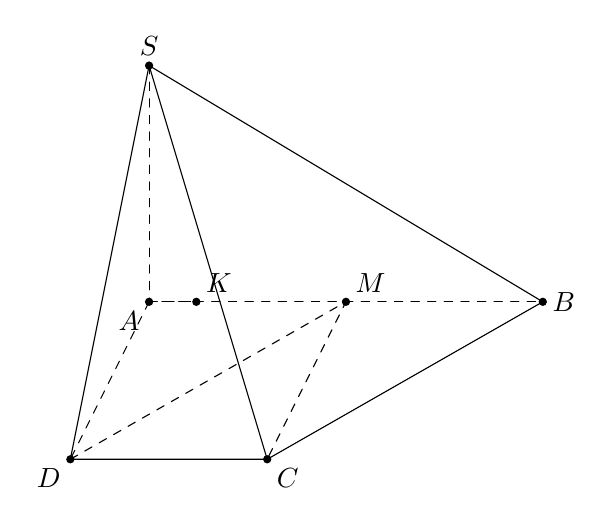
\begin{tikzpicture}[scale=1.0, line join=round, line cap=round]
				\coordinate (A) at (0,0);
				\coordinate (B) at (5,0);
				\coordinate (D) at (-1,-2);
				\coordinate (C) at (1.5,-2);
				\coordinate (M) at (2.5,0);
				\coordinate (S) at (0,3);
				\coordinate (K) at (0.6,0);
				\draw (S) -- (D) -- (C) -- (B) -- (S) -- (C);
				\draw[dashed] (S) -- (A) -- (B);
				\draw[dashed] (A) -- (D);
				\draw[dashed] (D) -- (M) -- (C);
				\draw[dashed] (A) -- (K);
				\fill (S) circle (1.5pt) node[above] {$S$};
				\fill (A) circle (1.5pt) node[below left] {$A$};
				\fill (B) circle (1.5pt) node[right] {$B$};
				\fill (C) circle (1.5pt) node[below right] {$C$};
				\fill (D) circle (1.5pt) node[below left] {$D$};
				\fill (M) circle (1.5pt) node[above right] {$M$};
				\fill (K) circle (1.5pt) node[above right] {$K$};
			\end{tikzpicture}
		\end{center}
		Ta có: $DM \parallel BC \Rightarrow DM \parallel (SBC)$\\
		nên $\displaystyle d(DM, SB) = d(DM, (SBC)) = d(M, (SBC)) = \frac{1}{2} d(A, (SBC))$.\\
		Nhận xét $CM = MB = BC = a \Rightarrow \Delta CMB$ đều nên $\widehat{ABC} = 60^\circ \Rightarrow \widehat{ADC} = 120^\circ$.\\
		Xét tam giác $\Delta ADC$ có $\displaystyle AC = \sqrt{AD^2 + DC^2 - 2AD \cdot DC \cdot \cos 120^\circ} = a\sqrt{3}$.\\
		Xét tam giác $\Delta ABC$ có $AC^2 + CB^2 = AB^2$ nên tam giác $\Delta ABC$ vuông tại $C$.\\
		Kẻ $AK \perp SC \Rightarrow AK \perp (SBC) \Rightarrow d(A, (SBC)) = AK$.\\
		Ta có $\displaystyle \frac{1}{AK^2} = \frac{1}{AC^2} + \frac{1}{SA^2} \Rightarrow AK = \frac{3}{2}a \Rightarrow d(DM, SB) = \frac{3}{4}a \Rightarrow \begin{cases} x = 3 \\ y = 4 \end{cases} \Rightarrow x + y + xy = 19$.
	}
\end{ex}

\begin{ex} %Câu 5. %[1D9C2-5]
	Trong một trò chơi thám hiểm, anh Sơn phải vượt qua một mê cung gồm các phòng thông nhau như sơ đồ dưới đây. Tại mỗi phòng, anh Sơn sẽ chọn ngẫu nhiên một trong các cửa thông với phòng hiện tại (với xác suất như nhau) để đi tiếp. Quá trình di chuyển diễn ra liên tục và trò chơi sẽ kết thúc ngay khi anh bước vào phòng chứa Kho báu hoặc phòng có Bẫy. Biết anh Sơn bắt đầu từ Phòng 1, tính xác suất để anh tìm được kho báu. (Kết quả làm tròn đến hàng phần trăm).
	\begin{center}
		\begin{tikzpicture}[scale=1.0]
			\draw[thick] (0,0) rectangle (6,4);
			\draw[thick] (3,0) -- (3,4);
			\draw[thick] (0,2) -- (6,2);
			\draw[thick] (2.5,3) -- (3.5,3);
			\draw[thick] (2.5,1) -- (3.5,1);
			\draw[thick] (1.5,1.5) -- (1.5,2.5);
			\draw[thick] (4.5,1.5) -- (4.5,2.5);
			\node at (1.5,3) {Phòng 1};
			\node at (4.5,3) {Phòng 2};
			\node at (1.5,1) {Phòng 3};
			\node at (4.5,1) {Phòng 4};
			\draw[thick] (-2,2) rectangle (0,4);
			\node at (-1,3) {Kho báu};
			\draw[thick] (6,0) rectangle (8,2);
			\node at (7,1) {Bẫy};
		\end{tikzpicture}
	\end{center}
	\shortans[oly]{$0{,}67$}
	\loigiai
	{
		Gọi $P_i$ là xác suất để anh Sơn tìm được kho báu nếu anh ấy đang đứng ở Phòng $i$ (với $i \in \{1, 2, 3, 4\}$). Ta cần tính $P_1$.\\
		Tại Phòng 1 có 3 cửa để đi (Kho báu, Phòng 2, Phòng 3). Xác suất chọn mỗi cửa là $\displaystyle \frac{1}{3}$. Nếu đi vào phòng Kho báu thì trò chơi kết thúc nên xác suất = 1. Do đó: $\displaystyle P_1 = \frac{1}{3} \cdot 1 + \frac{1}{3} P_2 + \frac{1}{3} P_3 \quad (1)$\\
		Tại Phòng 2 có 2 cửa để đi (Phòng 1, Phòng 4). Do đó: $\displaystyle P_2 = \frac{1}{2} P_1 + \frac{1}{2} P_4 \quad (2)$\\
		Tại Phòng 3 có 2 cửa để đi (Phòng 1, Phòng 4). Do đó: $\displaystyle P_3 = \frac{1}{2} P_1 + \frac{1}{2} P_4 \quad (3)$\\
		Tại Phòng 4 có 3 cửa để đi (Phòng 2, Phòng 3, Bẫy). Nếu đi vào phòng Bẫy thì trò chơi kết thúc nên xác suất = 0. Do đó: $\displaystyle P_4 = \frac{1}{3} P_2 + \frac{1}{3} P_3 \quad (4)$\\
		Từ (1), (2), (3), (4) ta có hệ phương trình:
		$\begin{cases} \displaystyle P_1 = \frac{1}{3} + \frac{2}{3} P_2 \\ \displaystyle P_2 = P_3 = \frac{1}{2} P_1 + \frac{1}{2} P_4 \\ \displaystyle P_4 = \frac{2}{3} P_2 \end{cases}$\\
		Giải hệ trên ta tìm được $\displaystyle P_1 = \frac{2}{3}, P_2 = P_3 = \frac{1}{2}, P_4 = \frac{1}{3}$. Vậy $\displaystyle P_1 = \frac{2}{3} \approx 0{,}67$.
	}
\end{ex}

\begin{ex} %Câu 6. %[0D8C2-5]
	Nhân dịp nghỉ lễ 30/4, siêu thị X in ra 100 phiếu thưởng được đánh số thứ tự từ 1 đến 100, mỗi phiếu ghi 1 số, các phiếu khác nhau ghi số khác nhau. Mỗi khách hàng trong 100 khách hàng đầu tiên đến siêu thị trong ngày 30/4 sẽ được nhận 1 phiếu thưởng. Những người được nhận phiếu thưởng có thể tìm thêm 2 người khác để ghép thành 1 nhóm có 3 người. Nếu tổng các số ghi trên 3 thẻ của 3 người trong nhóm bằng 100 thì mỗi người trong nhóm được nhận 50.000đ. Siêu thị quy định:\\
	1) Một người có thể ghép vào nhiều nhóm nên có thể nhận thưởng nhiều lần.\\
	2) Mỗi nhóm 3 người chỉ được nhận thưởng 1 lần.\\
	Hỏi ban quản lý siêu thị phải chuẩn bị số tiền thưởng lớn nhất là bao nhiêu triệu đồng (kết quả làm tròn đến hàng đơn vị)?
	\shortans[oly]{$118$}
	\loigiai
	{
		Vì mỗi nhóm 3 người được nhận thưởng 1 lần và mỗi người có thể tham gia nhiều nhóm nên tổng số tiền thưởng lớn nhất phụ thuộc hoàn toàn vào tổng số bộ 3 thẻ phân biệt có tổng bằng 100.\\
		Gọi $x, y, z$ là các số trên 3 thẻ, vì các thẻ phân biệt nên ta có thể giả sử $x < y < z$. Khi đó ta cần tìm số nghiệm nguyên của phương trình:\\
		$x + y + z = 100$\\
		Với điều kiện: $1 \le x, y, z \le 100$.\\
		Để tìm bộ 3 số $x, y, z$ thỏa mãn, ta dùng phương pháp phần bù.\\
		+ Đầu tiên, ta tính số bộ 3 $(x, y, z)$ thỏa mãn $x + y + z = 100$ (không có thứ tự và có thể giống nhau). Đây là bài toán chia kẹo Euler đã biết. Ta sắp xếp 100 cái kẹo thành hàng ngang, khi đó giữa chúng có 99 chỗ trống (không kể hai đầu). Dùng hai vách ngăn để chia các viên kẹo thành 3 phần. Suy ra số bộ 3 $(x, y, z)$ thỏa mãn là: $C_{99}^2$ bộ.\\
		+ Nếu $x = y = z$ thì $\displaystyle x + y + z = 100 \Leftrightarrow 3x = 100 \Leftrightarrow x = \frac{100}{3}$ (không thỏa mãn).\\
		+ Nếu $x = y \ne z$ thì $x + y + z = 100 \Leftrightarrow 2x + z = 100 \Leftrightarrow z = 100 - 2x = 2(50 - x)$.\\
		Do đó, $z$ là số chẵn $\Rightarrow z \in \{2; 4; 6; \dots; 98\}$ và với mỗi số $z$ có duy nhất một cách chọn $x = y$.\\
		Từ đó ta tính được có $\displaystyle \frac{98 - 2}{2} + 1 = 49$ bộ.\\
		+ Các trường hợp $x = z \ne y$ và $y = z \ne x$ làm tương tự như trên.\\
		Do đó số cách chọn các bộ số $(x, y, z)$ phân biệt thỏa mãn sẽ là: $C_{99}^2 - 3 \cdot 49 = 4704$ bộ.\\
		Tuy nhiên, vì có thêm điều kiện $x < y < z$ nên phải chia cho số hoán vị 3 phần tử $x, y, z$, tức là số bộ số $(x, y, z)$ thỏa mãn là: $\displaystyle \frac{4704}{3!} = 784$ bộ.\\
		Mỗi nhóm có 3 người, mỗi người nhận $50000\text{đ}$, nên mỗi nhóm nhận được $3 \cdot 50000 = 150000\text{ đồng}$. Do đó, tổng số tiền thưởng siêu thị phải chuẩn bị là:\\
		$784 \cdot 150000 = 117600000 \approx 118\text{ triệu đồng}$.
	}
\end{ex}

\Closesolutionfile{ans}

\indapan{6}{ans/ans-26-2--SoGD-L1-LC}
\indapan{4}{ans/ans-26-2--SoGD-L1-DS}
\indapan{6}{ans/ans-26-2--SoGD-L1-KQ}








